% !TEX root = task-3-18-1.tex
% Editable task bank. Append new BankTask blocks at the end of the document.
\documentclass[12pt,a4paper]{article}
\usepackage{physics-textbook}
\usepackage{graphicx,needspace}
\usetikzlibrary{decorations.pathmorphing}
\newif\ifShowSolutions
\ifdefined\TutorEdition
  \ShowSolutionstrue
\else
  \ShowSolutionsfalse % Change to \ShowSolutionstrue to display solutions.
\fi
\newcounter{banktask}
\newsavebox{\BankTaskBox}
\newcommand{\BankTaskContent}[3]{%
  \noindent\textbf{\thebanktask.}\quad #2\par
  \ifShowSolutions
    \Needspace{50mm}% Keep the solution heading with its opening text or diagram.
    #3\par
    \ifdefined\TutorEdition
      \ifcsname TutorSource#1\endcsname
        \nopagebreak\smallskip{\small\csname TutorSource#1\endcsname\par}%
      \fi
    \fi
  \fi
}
\newcommand{\BankTask}[3]{%
  \refstepcounter{banktask}\par\medskip
  \sbox{\BankTaskBox}{\begin{minipage}{\linewidth}%
    \BankTaskContent{#1}{#2}{#3}\end{minipage}}%
  \ifdim\dimexpr\ht\BankTaskBox+\dp\BankTaskBox\relax>\dimexpr\textheight-20mm\relax
    \Needspace{35mm}\BankTaskContent{#1}{#2}{#3}%
  \else
    \Needspace{\dimexpr\ht\BankTaskBox+\dp\BankTaskBox\relax}%
    \noindent\usebox{\BankTaskBox}\par
  \fi
  \medskip
}
\begin{document}
\BookSubsection{3.18.1}{Сила Лоренца}


% Source sdamgia-25793: https://phys-ege.sdamgia.ru/problem?id=25793
\BankTask{sdamgia-25793}{
\begin{center}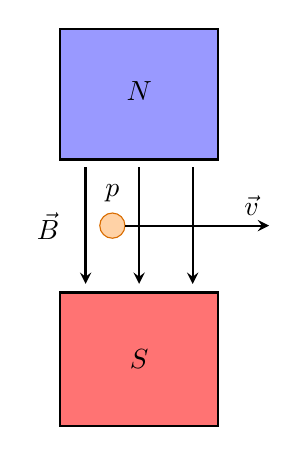
\begin{tikzpicture}[>=stealth]
\draw[thick,fill=blue!40] (-1,1.24) rectangle (1,2.9);
\draw[thick,fill=red!55] (-1,-2.14) rectangle (1,-.45);
\node at(0,2.11){$N$};\node at(0,-1.29){$S$};
\foreach \x in {-.68,0,.68}{\draw[->,thick] (\x,1.14)--(\x,-.34);}
\node[left]at(-.89,.4){$\vec B$};
\filldraw[fill=orange!35,draw=orange!85!black](-.34,.4)circle(.16);
\node[above]at(-.34,.58){$p$};
\draw[->,thick](-.18,.4)--(1.65,.4)node[above left]{$\vec v$};
\end{tikzpicture}\end{center}
Протон p влетает в зазор между полюсами электромагнита с горизонтальной скоростью $\vec v ,$ лежащей в плоскости рисунка. Вектор индукции $\vec{B}$ магнитного поля направлен вертикально. Куда направлена (вправо, влево, к наблюдателю, от наблюдателя) действующая на протон сила Лоренца?
}{
\smallskip\noindent\textbf{Решение}\par
По правилу левой руки: «Если левую руку расположить так, чтобы линии магнитной индукции входили в ладонь, а вытянутые четыре пальца совпадали с направлением движения заряда, то отогнутый большой палец укажет направление силы Лоренца, действующей на положительный заряд». Поскольку протон несет положительный заряд, мысленно проделав указанные действия, получаем, что сила Лоренца направлена от наблюдателя.

Ответ: от наблюдателя.
}

% Source sdamgia-25795: https://phys-ege.sdamgia.ru/problem?id=25795
\BankTask{sdamgia-25795}{
\begin{center}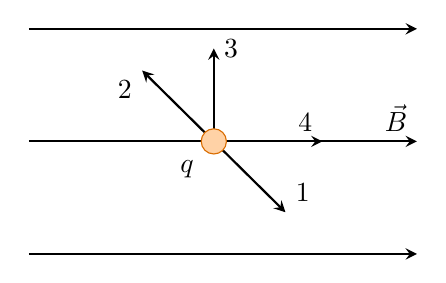
\begin{tikzpicture}[>=stealth]
\foreach \y in {-1.43,0,1.43}{\draw[->,thick](-2.35,\y)--(2.58,\y);}
\node[above left]at(2.58,0){$\vec B$};
\draw[->,thick] (0,0)--(1.38,0)node[above left]{$4$};
\draw[->,thick] (0,0)--(0,1.18)node[right]{$3$};
\draw[->,thick] (0,0)--(-.91,.9)node[below left]{$2$};
\draw[->,thick] (0,0)--(.91,-.9)node[above right]{$1$};
\filldraw[fill=orange!35,draw=orange!85!black](0,0)circle(.16);
\node[below left]at(-.13,-.12){$q$};
\end{tikzpicture}\end{center}
В каком направлении из предложенных на рисунке (вправо, вверх, к наблюдателю, от наблюдателя) нужно двигать в однородном магнитном поле $\vec{B}$ точечный заряд q для того, чтобы действующая на него сила Лоренца при одинаковой по модулю скорости этого движения была минимальной?
}{
\smallskip\noindent\textbf{Решение}\par
Величина силы Лоренца дается выражением $F_{\,\text{Л}}=q v B \sin \alpha ,$ где $\alpha$  —  угол между направлением поля и вектора скорости. Следовательно, для того, чтобы сила Лоренца была минимальна, заряд нужно двигать вдоль линий магнитного поля, то есть вправо.

Ответ: вправо.
}

% Source sdamgia-28087: https://phys-ege.sdamgia.ru/problem?id=28087
\BankTask{sdamgia-28087}{
В однородное магнитное поле перпендикулярно линиям индукции влетают с одинаковой скоростью протон и электрон. Определите отношение модулей этих сил Лоренца $\frac{F_e}{F_p} ,$ действующих на протон и электрон со стороны магнитного поля.
}{
\smallskip\noindent\textbf{Решение}\par
Сила Лоренца равна $F=Bqv \sin \alpha .$ Поскольку магнитная индукция поля одинакова, скорости заряженных частиц одинаковы, заряды протона и электрона по модулю одинаковы, угол между направлением скорости и вектором магнитной индукции прямой, то отношение модулей этих сил Лоренца $\frac{F_e}{F_p}$  =  $1$.

Ответ: $1$.
}

% Source sdamgia-41543: https://phys-ege.sdamgia.ru/problem?id=41543
\BankTask{sdamgia-41543}{
Протон p, имеющий скорость $v ,$ и нейтрон n, имеющий скорость $2 v ,$ влетают в однородное магнитное поле перпендикулярно вектору магнитной индукции. Определите отношение $\frac{F_n}{F_p}$ модулей сил, действующих со стороны магнитного поля на эти частицы.
}{
\smallskip\noindent\textbf{Решение}\par
Так как нейтрон не имеет заряда, то сила Лоренца со стороны магнитного поля не действует. Следовательно, отношение $\frac{F_n}{F_p} =0.$

Ответ: $0$.
}

% Source sdamgia-29987: https://phys-ege.sdamgia.ru/problem?id=29987
\BankTask{sdamgia-29987}{
Две частицы с зарядами $q_1=2 q$ и $q_2=q$ влетают в однородное магнитное поле перпендикулярно вектору магнитной индукции со скоростями $v _1= v$ и $v _2=2 v$ соответственно. Определите отношение модулей сил $F_1: F_2,$ действующих на них со стороны магнитного поля.
}{
\smallskip\noindent\textbf{Решение}\par
На заряженные частицы, движущиеся в магнитном поле, действует сила Лоренца $F_L=Bq v \sin \alpha .$ Тогда отношение сил, действующих на них со стороны магнитного поля, равно:

\[\frac{F_1}{F_2} = \frac{B \cdot 2q \cdot v}{B \cdot q \cdot 2 v} =1.\]

Ответ: $1$.
}

% Source sdamgia-3711: https://phys-ege.sdamgia.ru/problem?id=3711
\BankTask{sdamgia-3711}{
Электрон влетает в однородное магнитное поле с индукцией $5\,\text{Тл}$ со скоростью $1\,\text{км/с}$, направленной под некоторым углом к силовым линиям магнитного поля. Найдите все возможные значения модуля силы Лоренца, действующей на электрон. 

Справочные данные: элементарный электрический заряд $e=1{,}6 \cdot 10 ^{ - 19 } \,\text{Кл}.$

$1$)  $8 \cdot 10 ^{ - 16 } \,\text{Н}$
$2$)  от $0$ до $8 \cdot 10 ^{ - 16 } \,\text{Н}$
$3$)  от $0$ до $8 \cdot 10 ^{ - 19 } \,\text{Н}$
$4$)  Модуль силы может принимать любое значение
}{
\smallskip\noindent\textbf{Решение}\par
На движущийся в магнитном поле электрон действует сила Лоренца, величина которой, определяется соотношением $F_{\,\text{Л}}=e v B \sin \alpha ,$ где $\alpha$  —  угол между вектором скорости частицы и вектором магнитной индукции. 
Поскольку про угол $\alpha$ в условии ничего не ничего не сказано, необходимо рассмотреть все возможные его значения из отрезка $0 \leq \alpha \leq \pi .$ На этом промежутке синус угла пробегает все значения от $0$ до $1$. Таким образом, минимальное значение силы Лоренца равно нулю $F_{\,\text{Л}} ^{ min } =0,$ то есть магнитное поле на электрон вообще не действует. Это происходит, когда электрон летит вдоль линии магнитного поля ($\alpha =0$) или против нее ($\alpha = \pi$). Максимальное значение сила Лоренца достигает, когда электрон летит перпендикулярно силовым линиям: $F_{\,\text{Л}} ^{ max } =1{,}6 \cdot 10 ^{ - 19 } \,\text{Кл} \cdot 5\,\text{Тл} \cdot 1000\,\text{м/с} \cdot 1=8 \cdot 10 ^{ - 16 } \,\text{Н}.$

Правильный ответ указан под номером $2$.
}

% Source sdamgia-32729: https://phys-ege.sdamgia.ru/problem?id=32729
\BankTask{sdamgia-32729}{
Протон движется по окружности в однородном магнитном поле. Во сколько раз увеличится модуль ускорения протона, если его кинетическую энергию уменьшить в $4$ раза, а модуль индукции магнитного поля увеличить в $4$ раза?
}{
\smallskip\noindent\textbf{Решение}\par
На заряженную частицу, движущуюся в магнитном поле, действует сила Лоренца $F_L=Bq v ,$ которая по второму закону Ньютона является причиной ускорения $a= \frac{F_L}{m} .$ 
Зная кинетическую энергию частицы, можем найти ее скорость $E_{\,\text{к}}= \frac{m v ^2}{2} ,$ откуда $v = \sqrt{\frac{2E_{\,\text{к}}}{m}} .$ Тогда ускорение протона равно:

\[a= \frac{Bq}{m} \sqrt{\frac{2E_{\,\text{к}}}{m}} .\]

При увеличении модуля индукции магнитного поля в $4$ раза и уменьшении кинетической энергии протона ускорение увеличится в $2$ раза.

Ответ: $2$.
}

% Source sdamgia-25399: https://phys-ege.sdamgia.ru/problem?id=25399
\BankTask{sdamgia-25399}{
\begin{center}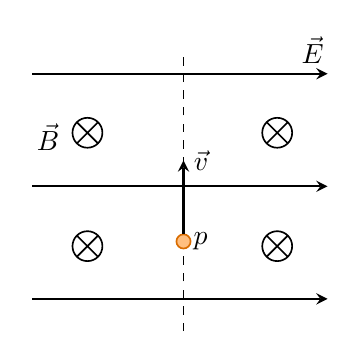
\begin{tikzpicture}[>=stealth,line width=.6pt]

\foreach \y in {-.9,.53,1.96}{\draw[->,thick](-1.68,\y)--(2.07,\y);}
\node[above]at(1.88,1.96){$\vec E$};
\foreach \x in {-.98,1.43}\foreach \y in {-.23,1.21}{\draw(\x,\y)circle(.19) (\x-.13,\y-.13)--(\x+.13,\y+.13) (\x-.13,\y+.13)--(\x+.13,\y-.13);}
\node[left]at(-1.21,1.15){$\vec B$};
\draw[dashed](.24,-1.31)--(.24,2.27);
\filldraw[fill=orange!50,draw=orange!85!black](.24,-.17)circle(.09) node[right]{$p$};
\draw[->,thick](.24,-.07)--(.24,.86)node[right]{$\vec v$};

\end{tikzpicture}\end{center}
В камере, из которой откачан воздух, создали электрическое поле напряженностью $\vec{E}$ и магнитное поле с индукцией $\vec{B}.$ Поля однородные, $\vec{E}\perp\vec{B}.$ В камеру влетает протон p, вектор скорости которого перпендикулярен $\overrightarrow{B}$ и $\overrightarrow{E}$ как показано на рисунке. Модули напряженности электрического поля и индукции магнитного поля таковы, что протон движется прямолинейно. Куда отклонится протон на начальном участке траектории, если его скорость уменьшить? Ответ поясните, указав, какие явления и закономерности Вы использовали для объяснения. Влиянием силы тяжести пренебречь.
}{
\smallskip\noindent\textbf{Решение}\par
На протон действует две силы: со стороны электрического поля $F_{\,\text{э}}=qE,$ направленная вправо, так как протон имеет положительный заряд; со стороны магнитного поля сила Лоренца $F_L=Bq v ,$ направленная влево по правилу левой руки. Протон движется равномерно, так как силы равны по модулю и противоположны, то есть равнодействующая этих сил равна $0$.
Если уменьшить скорость протона, то сила электрического поля не изменится, а сила Лоренца уменьшится. Тогда равнодействующая сила будет направлена вправо. Поскольку сила перпендикулярна скорости, то протон будет двигаться по криволинейной траектории, похожей на дугу окружности на начальном участке, отклоняясь вправо.
}

% Source sdamgia-25352: https://phys-ege.sdamgia.ru/problem?id=25352
\BankTask{sdamgia-25352}{
Ион с зарядом $q=3{,}2 \cdot 10 ^{ - 19 }$ Кл и массой $1{,}5 \cdot 10 ^{ - 25 }$ кг проходит ускоряющую разность потенциалов U. После он влетает в магнитное поле с индукцией B  =  $0{,}3\,\text{Тл}$ и движется в нем по окружности с радиусом R  =  $0{,}25\,\text{м}$. Найдите ускоряющую разность потенциалов U ($v_0$, $mg$ пренебрегаем).
}{
\smallskip\noindent\textbf{Решение}\par
Заряженная частица разгонялась электрическим полем, следовательно, работа поля равна изменению кинетической энергии иона $A=\Delta E_k.$ При этом $A=qU,$ $\Delta E_k= \frac{m v ^2}{2} ,$ откуда $qU= \frac{m v ^2}{2} .$ Магнитное поле действует на ион силой Лоренца $F_L=Bq v \sin \alpha ,$ причем угол равен $90^\circ$, так как частица движется по окружности. По второму закону Ньютона $F_L=ma,$ а центростремительное ускорение $a= \frac{v ^2}{R} .$ Тогда получаем, что скорость заряженной частицы равна $v = \frac{RBq}{m} .$
Тогда ускоряющая разность потенциалов:

$U= \frac{R^2 B^2 q}{2m}= \frac{0{,}25 ^2 \cdot 0{,}09 \cdot 3{,}2 \cdot 10 ^{ - 19 }}{2 \cdot 1{,}5 \cdot 10 ^{ - 25 }} =6000$ В.

Ответ: $6000\,\text{В}$.
}

% Source sdamgia-43128: https://phys-ege.sdamgia.ru/problem?id=43128
\BankTask{sdamgia-43128}{
\begin{center}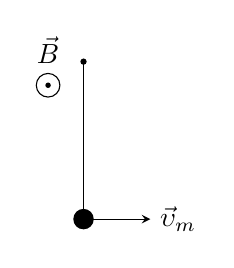
\begin{tikzpicture}[>=stealth]

\draw (0,2)--(0,0);\fill (0,2) circle(.04) (0,0) circle(.13);
\draw (-.45,1.7) circle(.15) node[above=.15cm]{$\vec B$};\fill (-.45,1.7) circle(.035);
\draw[->] (0,0)--(.85,0) node[right]{$\vec\upsilon_m$};
\end{tikzpicture}\end{center}
В однородном магнитном поле вращается по окружности в вертикальной плоскости положительно заряженный шарик массой m и зарядом q. Длина нити равна l. Минимальная скорость шарика в нижней точке, при которой шарик сможет совершить полный оборот, равна \ensuremath{\upsilon}. Найдите индукцию магнитного поля B.
}{
\smallskip\noindent\textbf{Решение}\par
\begin{center}\begin{tikzpicture}[>=stealth]

\draw (0,0) circle(1.4) (0,-1.4)--(0,1.4);\fill (0,-1.4) circle(.07) (0,0) circle(.05) (0,1.4) circle(.07);
\draw[->] (0,1.4)--(0,2.25) node[right]{$\vec F_{\!\text{л}}$};\draw[->] (0,1.4)--(0,.82) node[right]{$m\vec g$};
\draw[->] (0,.67)--(0,.29) node[right]{$\vec a$};\draw[->] (0,1.4)--(-.85,1.4) node[left]{$\vec\upsilon_2$};
\draw[->] (0,-1.4)--(.85,-1.4) node[right]{$\vec\upsilon_1$};\fill (-1.85,1.4) circle(.04) node[right]{$\vec B$};
\end{tikzpicture}\end{center}
При движении положительно заряженного тела магнитное поле действует на него с силой Лоренца, равной $F_{\,\text{л}}=Bq v \sin \alpha ,$ где $\sin \alpha =1,$ направление которой определяется правилом левой руки.
Рассмотрим движение заряженного шарика в магнитном и гравитационном поле. За нулевой уровень высоты примем нижнюю точку расположения шарика. В нижней точке он обладает кинетической энергией $E_{\,\text{к}1}= \frac{m v _1 ^2}{2} ,$  в верхней  — кинетической $E_{\,\text{к}2}= \frac{m v _2 ^2}{2}$ и потенциальной $E_{\,\text{п}2}=mgh=2mgl,$ где $v _2$ — скорость шарика в верхней точке. 
Так как сила Лоренца перпендикулярна вектору скорости, то работу не совершает. Тогда применим закон сохранения энергии:

\[\frac{m v _1 ^2}{2} = \frac{m v _2 ^2}{2} + 2mgl. ( 1 )\]

Так как шарику придали минимальную скорость, чтобы он совершил оборот в вертикальной плоскости, то в верхней точке сила натяжения нити равна $0$. На шарик в верхней точке действуют сила тяжести, сила Лоренца, направленная вверх. Под действием этих сил шарик имеет в верхней точке центростремительное ускорение $a= \frac{v _2 ^2}{R} = \frac{v _2 ^2}{l} .$
По второму закону Ньютона $m \vec{g} + \vec F_{\,\text{л}}=m \vec{a}.$ В проекции на вертикальную ось, направленную вниз получаем:

$mg - F_{\,\text{л}}=ma$
$Bq v _2=mg - \frac{m v _2 ^2}{l} . ( 2 )$

Объединяя формулы ($1$) и ($2$), находим индукцию магнитного поля:

\[B= \frac{m ( 5gl - v _1 ^2 )}{ql \sqrt{v _1 ^2 - 4gl}} .\]

Ответ: $B= \frac{m ( 5gl - v _1 ^2 )}{ql \sqrt{v _1 ^2 - 4gl}}$
}


% Source c0DF4F: https://ege.fipi.ru/bank/questions.php?search=1&proj=BA1F39653304A5B041B656915DC36B38&qid=c0DF4F
\BankTask{c0DF4F}{
Две частицы с зарядами \(q_1=2q\) и \(q_2=q\) влетают в однородное магнитное поле перпендикулярно вектору магнитной индукции со скоростями \(\upsilon_1=\upsilon\) и \(\upsilon_2=2\upsilon\) соответственно. Определите отношение \(\frac{F_1}{F_2}\) модулей сил, действующих на частицы со стороны магнитного поля в этот момент времени.
}{
\smallskip\noindent\textbf{Решение от GPT}\par
При движении перпендикулярно полю модуль силы Лоренца равен \(F=|q|\upsilon B\). Поэтому
\[
\frac{F_1}{F_2}=\frac{|2q|\upsilon B}{|q|\cdot2\upsilon B}=1.
\]
Ответ: \(1\).
}

% Source 4603AF: https://ege.fipi.ru/bank/questions.php?search=1&proj=BA1F39653304A5B041B656915DC36B38&qid=4603AF
\BankTask{4603AF}{
Две частицы с отношением зарядов $\frac{q_2}{q_1}=\frac{1}{8}$ движутся в однородных магнитных полях, перпендикулярных их скоростям: первая — в поле с индукцией $B_1$; вторая — в поле с индукцией $B_2$. Найдите отношение радиусов траекторий частиц $\frac{R_2}{R_1}$, если их импульсы одинаковы, а отношение модулей индукции $\frac{B_2}{B_1}=2$.
}{
\smallskip\noindent\textbf{Решение от GPT}\par
Радиус траектории $R=\frac{p}{|q|B}$. При одинаковых импульсах
\[
\frac{R_2}{R_1}=\frac{|q_1|B_1}{|q_2|B_2}=8\cdot\frac{1}{2}=4.
\]
Ответ: $4$.
}

% Source D798EB: https://ege.fipi.ru/bank/questions.php?search=1&proj=BA1F39653304A5B041B656915DC36B38&qid=D798EB
\BankTask{D798EB}{
Две частицы с отношением масс $\frac{m_2}{m_1}=4$ движутся в однородных магнитных полях, перпендикулярных их скоростям: первая — в поле с индукцией $\vec{B}_1$; вторая — в поле с индукцией $\vec{B}_2$. Найдите отношение времён $\frac{T_2}{T_1}$, затраченных частицами на один оборот, если их импульсы одинаковы, а отношение радиусов траекторий $\frac{R_2}{R_1}=\frac{1}{2}$.
}{
\smallskip\noindent\textbf{Решение от GPT}\par
Из $p=mv$ и $T=\frac{2\pi R}{v}$ получаем $T=\frac{2\pi Rm}{p}$. При одинаковых импульсах
\[
\frac{T_2}{T_1}=\frac{R_2}{R_1}\frac{m_2}{m_1}=\frac{1}{2}\cdot4=2.
\]
Ответ: $2$.
}

% Source DDF127: https://ege.fipi.ru/bank/questions.php?search=1&proj=BA1F39653304A5B041B656915DC36B38&qid=DDF127
\BankTask{DDF127}{
В первой экспериментальной установке положительно заряженная частица влетает в однородное электрическое поле так, что вектор $\vec{\upsilon}_0$ перпендикулярен вектору напряжённости электрического поля $\vec{E}$ (рис. 1). Во второй экспериментальной установке вектор $\vec{\upsilon}_0$ такой же частицы параллелен вектору индукции магнитного поля $\vec{B}$ (рис. 2).

По каким траекториям движутся частицы в этих установках? Силу тяжести не учитывать.

\TaskMatchingColumns[0.47\linewidth]{Движение частицы}{
А) в первой установке\par
Б) во второй установке
}{Траектория}{
1) прямая линия\par
2) окружность\par
3) спираль\par
4) парабола
}

\begin{center}
\begin{tabular}{|c|c|}
\hline
А & Б \\
\hline
\phantom{0} & \phantom{0} \\
\hline
\end{tabular}
\end{center}

\begin{center}
\begin{tikzpicture}[book diagram,line cap=round,line join=round]
\begin{scope}[x=0.65cm,y=0.65cm]
\foreach \x in {0,1,2,3,4,5}{
  \foreach \y in {0,1,2,3,4,5}{
    \draw (\x,\y) circle[radius=0.20];
    \fill (\x,\y) circle[radius=0.035];
  }
}
\draw[fill=white] (3.37,2.52) circle[radius=0.23];
\node at (3.37,2.52) {$+$};
\draw[-{book tip}] (2.33,2.52)--(3.03,2.52);
\node[above] at (2.67,2.59) {$\vec{\upsilon}_0$};
\node at (5.58,3.55) {$\vec E$};
\node at (2.5,-0.65) {Рис. 1};
\end{scope}
\begin{scope}[shift={(5.4cm,0cm)},x=0.65cm,y=0.65cm]
\foreach \x in {0,1.2,2.4}{
  \draw[-{book tip}] (\x,0.4)--(\x,4.75);
}
\draw[fill=white] (0.45,2.75) circle[radius=0.23];
\node at (0.45,2.75) {$+$};
\draw[-{book tip}] (0.45,2.46)--(0.45,1.78);
\node[right] at (0.48,2.03) {$\vec{\upsilon}_0$};
\node[right] at (2.45,4.75) {$\vec B$};
\node at (1.2,-0.65) {Рис. 2};
\end{scope}
\end{tikzpicture}
\end{center}
}{
\smallskip\noindent\textbf{Решение от GPT}\par
В первой установке постоянная сила $\vec F=q\vec E$ сообщает частице ускорение, перпендикулярное начальной скорости: $x=\upsilon_0t$, $z=qEt^2/(2m)$, поэтому траектория --- парабола (4). Во второй установке $\vec\upsilon_0$ антипараллелен $\vec B$, как показано на рисунке, поэтому $F_{\text{Л}}=q\upsilon B\sin180^\circ=0$ и частица движется по прямой (1). Окружность (2) требует поперечной магнитной силы, а спираль (3) --- одновременно ненулевых продольной и поперечной составляющих скорости в магнитном поле; здесь этих условий нет. Ответ: А --- 4, Б --- 1.
}

% Source AE92AD: https://ege.fipi.ru/bank/questions.php?search=1&proj=BA1F39653304A5B041B656915DC36B38&qid=AE92AD
\BankTask{AE92AD}{
В первой экспериментальной установке положительно заряженная частица влетает в однородное электрическое поле так, что вектор скорости $\vec{\upsilon}_0$ частицы параллелен вектору напряжённости электрического поля $\vec{E}$ (рис. 1). Во второй установке вектор скорости $\vec{\upsilon}_0$ отрицательно заряженной частицы перпендикулярен вектору индукции магнитного поля $\vec{B}$ (рис. 2).

По каким траекториям движутся частицы в этих установках? Силой тяжести пренебречь.

\TaskMatchingColumns[0.47\linewidth]{Движение частицы}{
А) в первой установке\par
Б) во второй установке
}{Траектория}{
1) прямая линия\par
2) окружность\par
3) спираль\par
4) парабола
}

\begin{center}
\begin{tabular}{|c|c|}
\hline
А & Б \\
\hline
\phantom{0} & \phantom{0} \\
\hline
\end{tabular}
\end{center}

\begin{center}
\begin{tikzpicture}[book diagram,line cap=round,line join=round]
\begin{scope}[x=0.70cm,y=0.70cm]
\foreach \x in {0,1.2,2.4}{
  \draw[-{book tip}] (\x,4.4)--(\x,0);
}
\draw[fill=white] (0.45,2.35) circle[radius=0.23];
\node at (0.45,2.35) {$+$};
\draw[-{book tip}] (0.45,2.64)--(0.45,3.30);
\node[right] at (0.47,3.05) {$\vec{\upsilon}_0$};
\node[right] at (2.45,4.35) {$\vec E$};
\node at (1.2,-0.65) {Рис. 1};
\end{scope}
\begin{scope}[shift={(4.5cm,0.45cm)},x=0.70cm,y=0.70cm]
\foreach \x in {0,1.6,3.2}{
  \foreach \y in {0,1.6,3.2}{
    \draw (\x-0.25,\y-0.25)--(\x+0.25,\y+0.25);
    \draw (\x-0.25,\y+0.25)--(\x+0.25,\y-0.25);
  }
}
\draw[fill=white] (1.10,2.40) circle[radius=0.30];
\node at (1.10,2.40) {$-$};
\draw[-{book tip}] (1.43,2.40)--(3.05,2.40);
\node[above] at (2.30,2.50) {$\vec{\upsilon}_0$};
\node[right] at (3.45,0.80) {$\vec B$};
\node at (1.6,-1.29) {Рис. 2};
\end{scope}
\end{tikzpicture}
\end{center}
}{
\smallskip\noindent\textbf{Решение от GPT}\par
В первой установке сила $\vec F=q\vec E$ направлена вдоль той же прямой, что и начальная скорость, поэтому траектория --- прямая (1), в том числе после возможной остановки и движения обратно. Во второй установке сила Лоренца перпендикулярна скорости и служит центростремительной: $|q|\upsilon B=m\upsilon^2/r$, поэтому траектория --- окружность (2). Спирали (3) нет, поскольку отсутствует составляющая скорости вдоль магнитного поля; параболы (4) нет, поскольку в первой установке отсутствует начальная поперечная скорость. Ответ: А --- 1, Б --- 2.
}

% Source D0C61D: https://ege.fipi.ru/bank/questions.php?search=1&proj=BA1F39653304A5B041B656915DC36B38&qid=D0C61D
\BankTask{D0C61D}{
Протон массой $m$ и зарядом $q$ движется перпендикулярно линиям индукции однородного магнитного поля $\vec{B}$ по окружности со скоростью $\upsilon$. Действием силы тяжести пренебречь.

Установите соответствие между физическими величинами и формулами, по которым их можно рассчитать.

\TaskMatchingColumns[0.53\linewidth]{Физические величины}{
А) модуль ускорения протона\par
Б) период обращения протона по окружности
}{Формулы}{
1) $q\upsilon B$\par
2) $\dfrac{m\upsilon}{qB}$\par
3) $\dfrac{2\pi m}{qB}$\par
4) $\dfrac{q\upsilon B}{m}$
}

\begin{center}
\begin{tabular}{|c|c|}
\hline
А & Б \\
\hline
\phantom{4} & \phantom{3} \\
\hline
\end{tabular}
\end{center}
}{
\smallskip\noindent\textbf{Решение от GPT}\par
Сила Лоренца $F_{\text{Л}}=q\upsilon B$ сообщает протону ускорение $a=F_{\text{Л}}/m=q\upsilon B/m$, поэтому А соответствует формуле 4. Из $m\upsilon^2/r=q\upsilon B$ получаем $r=m\upsilon/(qB)$ и $T=2\pi r/\upsilon=2\pi m/(qB)$, поэтому Б соответствует формуле 3. Формулы 1 и 2 определяют соответственно силу и радиус окружности. Ответ: $43$.
}

% Source CB965A: https://ege.fipi.ru/bank/questions.php?search=1&proj=BA1F39653304A5B041B656915DC36B38&qid=CB965A
\BankTask{CB965A}{
Протон массой $m$ и зарядом $q$ движется перпендикулярно линиям индукции однородного магнитного поля $\vec{B}$ по окружности со скоростью $\upsilon$. Действием силы тяжести пренебречь.

Установите соответствие между физическими величинами и формулами, по которым их можно рассчитать.

\TaskMatchingColumns[0.53\linewidth]{Физические величины}{
А) радиус окружности, по которой движется протон\par
Б) модуль силы, действующей на протон со стороны магнитного поля
}{Формулы}{
1) $\dfrac{2\pi m}{qB}$\par
2) $\dfrac{m\upsilon}{qB}$\par
3) $\dfrac{2\pi B}{\upsilon}$\par
4) $q\upsilon B$
}

\begin{center}
\begin{tabular}{|c|c|}
\hline
А & Б \\
\hline
\phantom{2} & \phantom{4} \\
\hline
\end{tabular}
\end{center}
}{
\smallskip\noindent\textbf{Решение от GPT}\par
При движении перпендикулярно магнитному полю сила Лоренца равна $F_{\text{Л}}=q\upsilon B$, поэтому Б соответствует формуле 4. Из равенства $m\upsilon^2/r=q\upsilon B$ находим $r=m\upsilon/(qB)$, поэтому А соответствует формуле 2. Формула 1 определяет период обращения, а формула 3 не определяет ни радиус, ни силу. Ответ: $24$.
}

% Source 29880: https://phys-ege.sdamgia.ru/problem?id=29880
\BankTask{29880}{
\begin{center}\begin{tikzpicture}[>=stealth,line width=.55pt]\draw(0,-.48)arc(-140:-68:1.35) (-.3,-.13)arc(-140:-68:1);\draw[orange!85!black,->](1.41,-1.06)arc(-65:-159:1.15);\draw[->,orange!85!black](2.9,-1.07)--(1.6,-1.07);\draw(2.93,-1.34)rectangle(3.97,-.83)node[pos=.5]{И. Ч.};\draw(.1,-.58)--(.1,-1.87)--(5.03,-1.87)--(5.03,-.96) (-.18,-.31)--(5.03,-.31)--(5.03,-.63);\draw(5.03,-.7)circle(.07) (5.03,-.88)circle(.07);\node[right]at(5.12,-.8){$U$};\end{tikzpicture}\end{center}На рисунке показана схема устройства для предварительного отбора заряженных частиц для последующего детального исследования. Устройство представляет собой конденсатор, пластины которого изогнуты дугой радиусом $R.$ Перед попаданием в это пространство молекулы теряют один электрон. Во сколько раз надо изменить напряжение на обкладках конденсатора, чтобы сквозь него пролетали ионы, потерявшие два электрона? Влиянием силы тяжести пренебречь.
}{
\smallskip\noindent\textbf{Решение}\par
Центростремительное ускорение иона в конденсаторе $a= \frac{v ^2}{R}$ задается силой $F=qE= \frac{qU}{d}$ действия электрического поля, так что $\frac{qU}{d} =m \frac{v ^2}{R}$ (здесь q, m и \ensuremath{\upsilon} — соответственно заряд, масса и скорость иона; U  — напряжение на обкладках конденсатора, d  — расстояние между пластинами).
Тогда данное выражение имеет вид для каждого случая: 

$\frac{m v ^2}{R} = \frac{qU_1}{d}$ и $\frac{m v ^2}{R} = \frac{2qU_2}{d}$

Из соотношения видно, что для отбора ионов, потерявших два электрона, напряжение нужно уменьшить в $2$ раза.

Ответ:уменьшить в $2$ раза.
}

\end{document}
